

\tikzset{every picture/.style={line width=0.75pt}} %set default line width to 0.75pt        

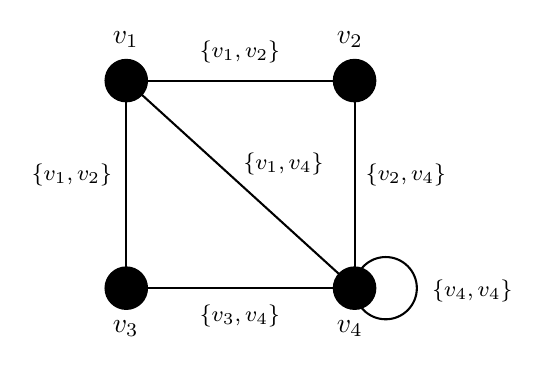
\begin{tikzpicture}[x=0.75pt,y=0.75pt,yscale=-1,xscale=1]
%uncomment if require: \path (0,178); %set diagram left start at 0, and has height of 178

%Shape: Circle [id:dp07024740871786728] 
\draw  [color={rgb, 255:red, 0; green, 0; blue, 0 }  ,draw opacity=1 ][fill={rgb, 255:red, 0; green, 0; blue, 0 }  ,fill opacity=1 ] (70,40) .. controls (70,34.48) and (74.48,30) .. (80,30) .. controls (85.52,30) and (90,34.48) .. (90,40) .. controls (90,45.52) and (85.52,50) .. (80,50) .. controls (74.48,50) and (70,45.52) .. (70,40) -- cycle ;
%Shape: Circle [id:dp433131734933478] 
\draw  [color={rgb, 255:red, 0; green, 0; blue, 0 }  ,draw opacity=1 ][fill={rgb, 255:red, 0; green, 0; blue, 0 }  ,fill opacity=1 ] (180,140) .. controls (180,134.48) and (184.48,130) .. (190,130) .. controls (195.52,130) and (200,134.48) .. (200,140) .. controls (200,145.52) and (195.52,150) .. (190,150) .. controls (184.48,150) and (180,145.52) .. (180,140) -- cycle ;
%Straight Lines [id:da2632273187556222] 
\draw    (80,40) -- (190,40) ;
%Straight Lines [id:da44290236983487796] 
\draw    (80,40) -- (80,140) ;
%Straight Lines [id:da1506700219779713] 
\draw    (80,40) -- (190,140) ;
%Straight Lines [id:da22133122848697484] 
\draw    (190,140) -- (190,40) ;
%Straight Lines [id:da5021664543420994] 
\draw    (80,140) -- (190,140) ;
%Shape: Circle [id:dp5653232034601401] 
\draw  [color={rgb, 255:red, 0; green, 0; blue, 0 }  ,draw opacity=1 ][fill={rgb, 255:red, 0; green, 0; blue, 0 }  ,fill opacity=1 ] (180,40) .. controls (180,34.48) and (184.48,30) .. (190,30) .. controls (195.52,30) and (200,34.48) .. (200,40) .. controls (200,45.52) and (195.52,50) .. (190,50) .. controls (184.48,50) and (180,45.52) .. (180,40) -- cycle ;
%Shape: Circle [id:dp644957096812665] 
\draw   (190,140) .. controls (190,131.72) and (196.72,125) .. (205,125) .. controls (213.28,125) and (220,131.72) .. (220,140) .. controls (220,148.28) and (213.28,155) .. (205,155) .. controls (196.72,155) and (190,148.28) .. (190,140) -- cycle ;
%Shape: Circle [id:dp5636675532432875] 
\draw  [color={rgb, 255:red, 0; green, 0; blue, 0 }  ,draw opacity=1 ][fill={rgb, 255:red, 0; green, 0; blue, 0 }  ,fill opacity=1 ] (70,140) .. controls (70,134.48) and (74.48,130) .. (80,130) .. controls (85.52,130) and (90,134.48) .. (90,140) .. controls (90,145.52) and (85.52,150) .. (80,150) .. controls (74.48,150) and (70,145.52) .. (70,140) -- cycle ;

% Text Node
\draw (72,15) node [anchor=north west][inner sep=0.75pt]    {$v_{1}$};
% Text Node
\draw (180,15) node [anchor=north west][inner sep=0.75pt]    {$v_{2}$};
% Text Node
\draw (72,154) node [anchor=north west][inner sep=0.75pt]    {$v_{3}$};
% Text Node
\draw (180,154) node [anchor=north west][inner sep=0.75pt]    {$v_{4}$};
% Text Node
\draw (114,19.4) node [anchor=north west][inner sep=0.75pt]  [font=\footnotesize]  {$\{v_{1} ,v_{2}\}$};
% Text Node
\draw (135,73.4) node [anchor=north west][inner sep=0.75pt]  [font=\footnotesize]  {$\{v_{1} ,v_{4}\}$};
% Text Node
\draw (194,78.4) node [anchor=north west][inner sep=0.75pt]  [font=\footnotesize]  {$\{v_{2} ,v_{4}\}$};
% Text Node
\draw (33,78.4) node [anchor=north west][inner sep=0.75pt]  [font=\footnotesize]  {$\{v_{1} ,v_{2}\}$};
% Text Node
\draw (114,146.4) node [anchor=north west][inner sep=0.75pt]  [font=\footnotesize]  {$\{v_{3} ,v_{4}\}$};
% Text Node
\draw (226,134.4) node [anchor=north west][inner sep=0.75pt]  [font=\footnotesize]  {$\{v_{4} ,v_{4}\}$};


\end{tikzpicture}